\insertmeeting 
	{More CAD} 
	{10-27-22}
	{Hagerty High School}
	{Jensen}
	{Images/RobotPics/robot.jpg}
	{4:30 - 7:30}
	
\hhscommittee{Hardware}
\noindent\hfil\rule{\textwidth}{.4pt}\hfil
\subsubsection*{Goals}
\begin{itemize}
    \item Discuss drivetrain

\end{itemize} 

\noindent\hfil\rule{\textwidth}{.4pt}\hfil

\subsubsection*{Accomplishments}
During today's meeting, we had a discussion about the efficiency of our car based drivetrain. To justify our use of the drivetrain we wanted to use similar justification to that of last year. Last year, we were able to justify our tricycle drivetrain because there were only curves that we had to make on the Freight Frenzy game field. This year there is more of a grid which means we need to make less significant arcs. To show the true benefit of our drivetrain we divided the field into smaller sections to show how we could use arcs in order to effectively maneuver the field without having any conflict with efficiency. This is helpful because during the early stages of development of our design we can strategize and figure out how our robot will need to move during matches. This reduces the need to experiment as when we begin driver practice we will already have basic strategies for driving. Sticking with the drivetrain design from last year also means that we have a strong understanding of the drivetrain and do not need to do as much practicing. Though our drivetrain cannot strafe like other drivetrains, we have a much lighter drivetrain and overall robot. Much like last year, we wanted to keep the robot fast and light so we could be as efficient as possible on the straightaways. This means that we will be able to better move from the close side of the field to the far side of the field. Another benefit of having a lighter robot is less influence on the arm. We ensured that majority of the weight on our robot was towards the bottom. We did this by keeping our motors towards the bottom and not moving a full motor on our track system which makes it lighter as it moves upwards. This means that our cart system is more accurate as the weight is more low to the ground lessening our center of gravity.
Next on the Docket: Creation of our drivetrain and proper testing.

\begin{figure}[htp]
\centering
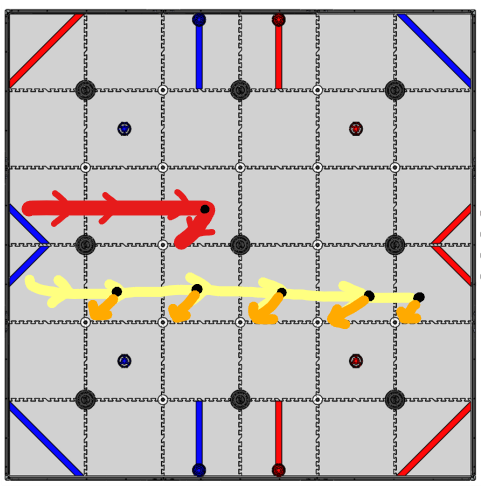
\includegraphics[width=0.9\textwidth, angle=0]{Meetings/October/10-27-22/10-27-22-Path.png}
\caption{Drive path.}
\label{fig:102722_1}
\end{figure}

\whatsnext{
\begin{itemize}
    \item Assemble our robot field parts
    
\end{itemize} 
}
